% \documentclass[handout]{beamer}
\documentclass{beamer}

\mode<presentation>
{
  \usetheme{default}
  \usefonttheme[onlymath]{serif}
  % \usetheme{Singapore}
  % \usetheme{Warsaw}
  % \usetheme{Malmoe}
  % \useinnertheme{circles}
  % \useoutertheme{infolines}
  % \useinnertheme{rounded}

  \setbeamercovered{transparent=100}
}

\usepackage[english]{babel}
\usepackage[latin1]{inputenc}
\usepackage{alltt,listings,multirow,ulem,siunitx}
\usepackage[absolute,overlay]{textpos}
\TPGrid{1}{1}
\usepackage{pdfpages}
\usepackage{multimedia}
\usepackage{multicol}
\newcommand\hmmax{0}
\newcommand\bmmax{0}
\usepackage{bm}

% font definitions, try \usepackage{ae} instead of the following
% three lines if you don't like this look
\usepackage{mathptmx}
\usepackage[scaled=.90]{helvet}
% \usepackage{courier}
\usepackage[T1]{fontenc}
\usepackage{tikz}
\usetikzlibrary{decorations.pathreplacing}
\usetikzlibrary{shadows,arrows,shapes.misc,shapes.arrows,shapes.multipart,arrows,decorations.pathmorphing,backgrounds,positioning,fit,petri,calc,shadows,chains,matrix}


% \usepackage{pgfpages}
% \pgfpagesuselayout{4 on 1}[a4paper,landscape,border shrink=5mm]

\usepackage{JedMacros}

\title{Pervasive Multiscale Modeling, Analysis, and Solvers}
\author{{\bf Jed Brown}}

% - Use the \inst command only if there are several affiliations.
% - Keep it simple, no one is interested in your street address.
\institute
{
  {Mathematics and Computer Science Division, Argonne National Laboratory} \\
}

\date{MathGeo, Princeton, 2012-10-02}

% This is only inserted into the PDF information catalog. Can be left
% out.
\subject{Talks}


% If you have a file called "university-logo-filename.xxx", where xxx
% is a graphic format that can be processed by latex or pdflatex,
% resp., then you can add a logo as follows:

% \pgfdeclareimage[height=0.5cm]{university-logo}{university-logo-filename}
% \logo{\pgfuseimage{university-logo}}



% Delete this, if you do not want the table of contents to pop up at
% the beginning of each subsection:
% \AtBeginSubsection[]
% {
% \begin{frame}<beamer>
%   \frametitle{Outline}
%   \tableofcontents[currentsection,currentsubsection]
% \end{frame}
% }

\AtBeginSection[]
{
  \begin{frame}<beamer>
    \frametitle{Outline}
    \tableofcontents[currentsection]
  \end{frame}
}

% If you wish to uncover everything in a step-wise fashion, uncomment
% the following command:

% \beamerdefaultoverlayspecification{<+->}

\begin{document}
\lstset{language=C}
\normalem

\begin{frame}
  \titlepage
\end{frame}

\begin{frame}{Motivation}
  \begin{itemize}
  \item Nature has many spatial and temporal scales
    \begin{itemize}
    \item Porous media, turbulence, kinetics, fracture
    \end{itemize}
  \item Robust discretizations and implicit solvers are needed to cope
  \item Computer architecture is increasingly hierarchical
    \begin{itemize}
    \item algorithms should conform to this structure
    \end{itemize}
  \item Solver scalability is a crucial bottleneck at scale
  \item ``black box'' solvers are not sustainable
    \begin{itemize}
    \item optimal solvers must accurately handle all scales
    \item optimality is crucial for large-scale problems
    \item hardware puts up a spirited fight to abstraction
    \end{itemize}
  \end{itemize}
\end{frame}

\begin{frame}
  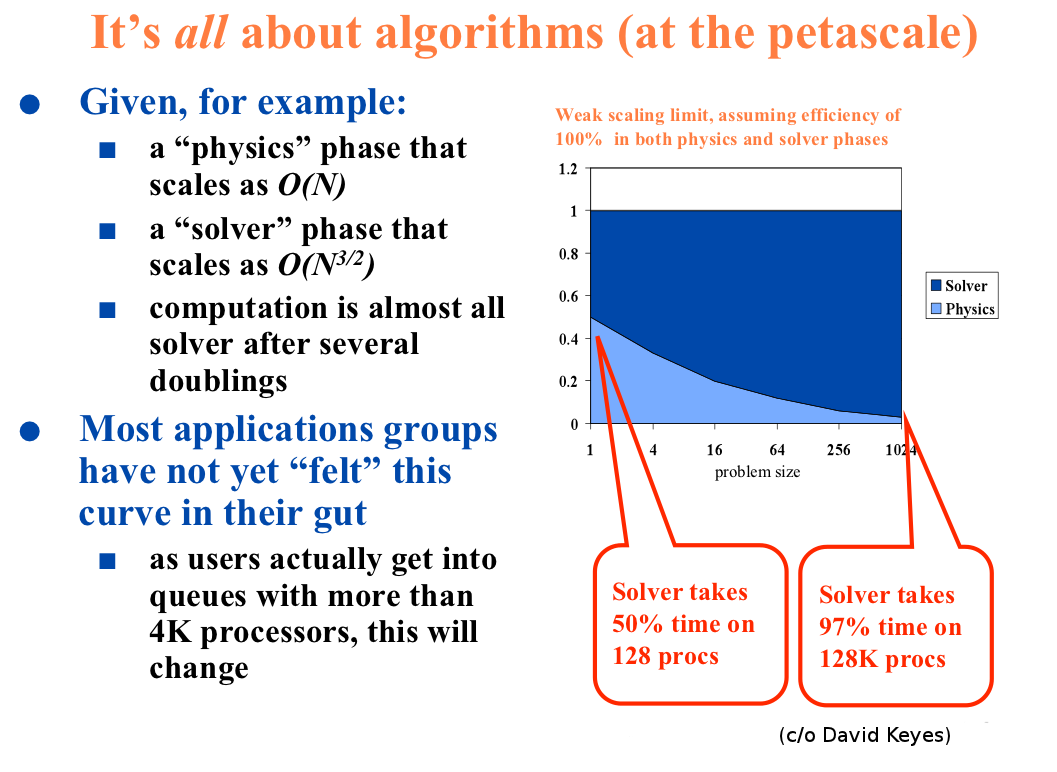
\includegraphics[width=1.05\textwidth]{figures/KeyesAllAboutAlgorithms}
\end{frame}

\begin{frame}{Phenomenological Models}
  \begin{quote}
    With four parameters I can fit an elephant, and with five I can make him wiggle his trunk. --- John von Neumann
  \end{quote}
  \vspace{-1ex}
  \begin{multicols}{2}
    \begin{itemize}
    \item Over-fitting is a pathology
    \item \emph{Good} subgrid models do not require re-tuning parameters
    \item Fracture
    \item Turbulence modeling
    \end{itemize}
  \end{multicols}
  \begin{quote}
    A professional problem exists %in the computational fluid dynamics community and also in the broader area of computational physics. Namely,
[...] there is a need for higher standards on the control of numerical accuracy. [...] it was impossible to evaluate and compare the accuracy of different turbulence models, since one could not distinguish physical modeling errors from numerical errors related to the algorithm and grid. [...] The Journal of Fluids Engineering {\bf will not accept for publication any paper}
% reporting the numerical solution of a fluids engineering problem
[...] that fails to address the task of {\bf systematic truncation error testing and accuracy estimation}. --- 1986
  \end{quote}
\end{frame}

{
\usebackgroundtemplate{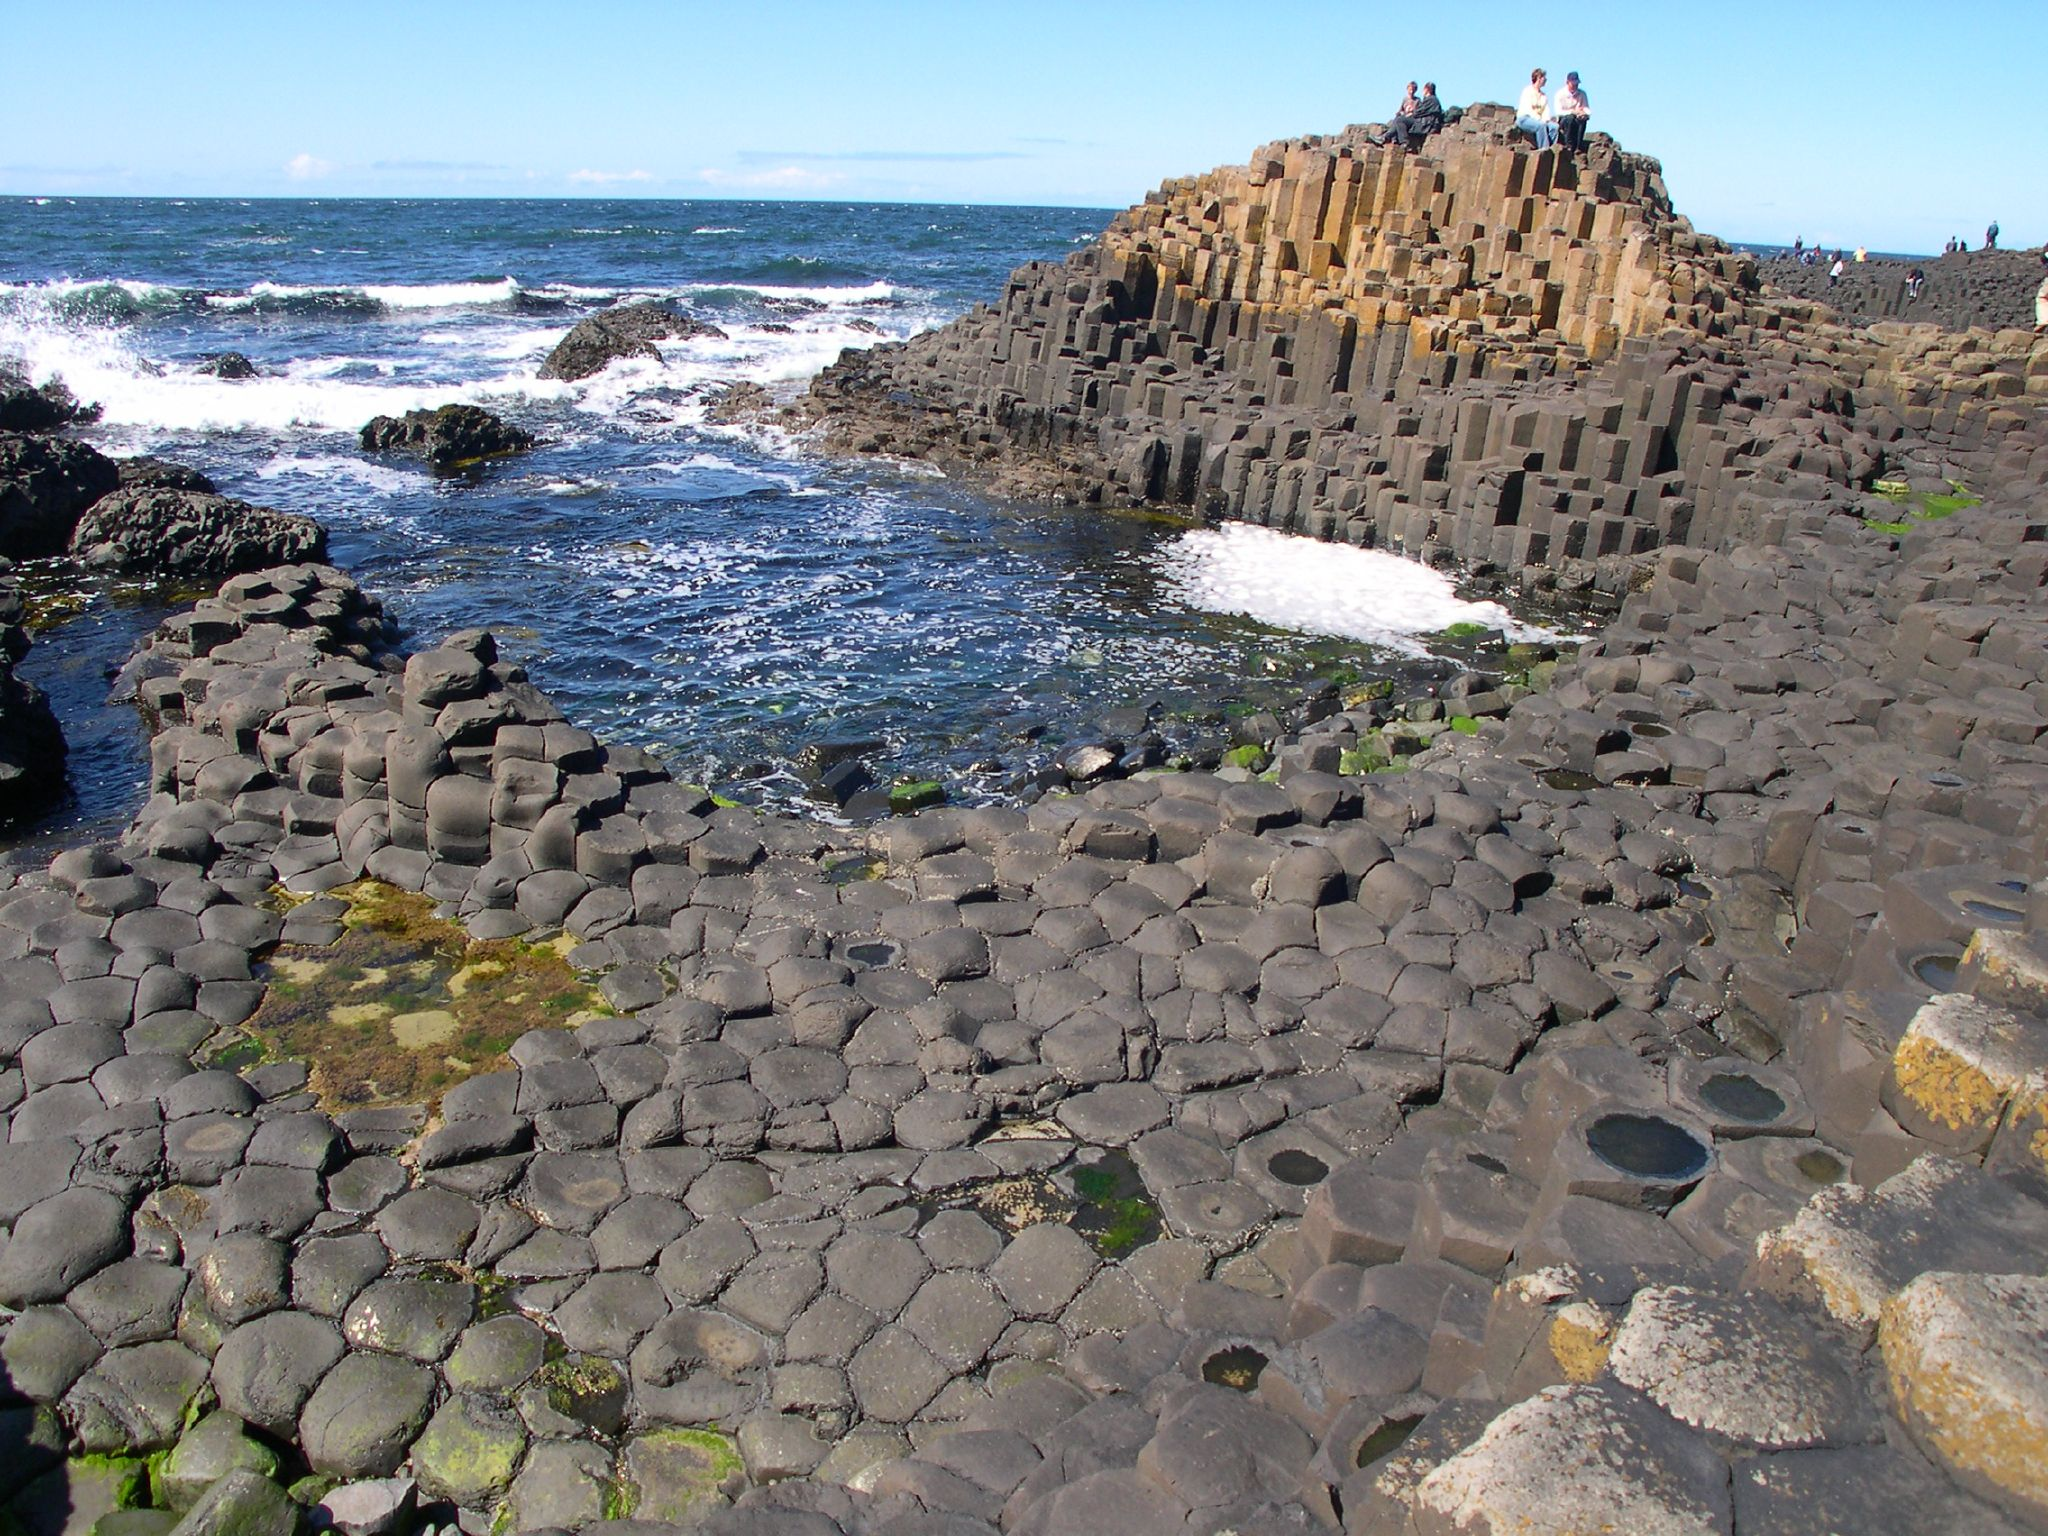
\includegraphics[width=\paperwidth]{figures/GiantsCauseway}}%
\begin{frame}{Diffusive cooling}
  \begin{textblock}{0.5}[1,0](0.99,0.1)
    \textblockcolour{black}
    \begin{itemize} \color{white} \small
    \item Pentagonal structures occur only for narrow band of thermal conditions and composition
    \item Variational (phase-field) approach reproduces thresholds without tuning [Bourdin, Francfort, Marigo]
    \end{itemize}
    %\movie{\includegraphics[width=\textwidth]{CoolingFrame.jpg}}{Cooling.mov}
    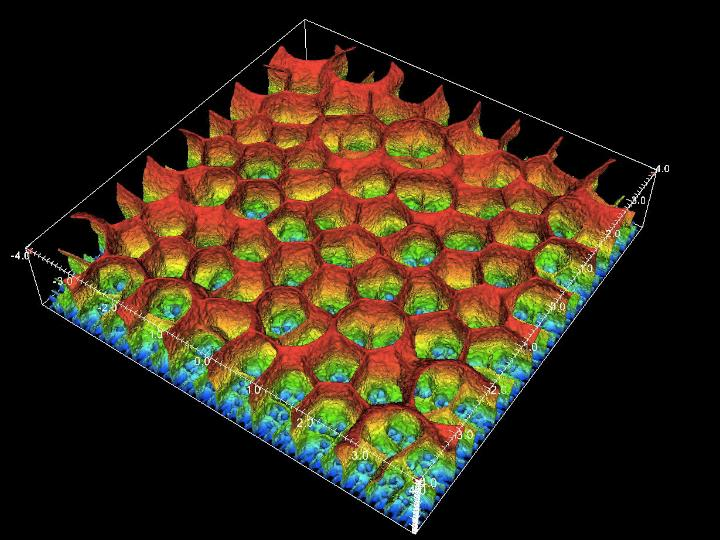
\includegraphics[width=\textwidth]{figures/BlaiseCoolingFrame.jpg}
  \end{textblock}
  % \begin{columns}
  %   \begin{column}{0.5\textwidth}
  %   \end{column}
  %   \begin{column}{0.5\textwidth}
  %   
  %   \end{column}
  % \end{columns}
\end{frame}
}

\begin{frame}{Numerical Homogenization/Upscaling}
  \begin{enumerate}
  \item Multiscale basis functions
    \begin{itemize}
    \item integrate against microscale coefficients
    \item robust theory for linear elliptic equations
    \item popular in porous media and composite materials
    \item practically computable using multigrid ideas, partition of unity method
    \item no support for stochastic microscale
    \end{itemize}
  \item Coefficient/equation upscaling
    \begin{itemize}
    \item a good method reproduces statistics
    \item cannot recover fine grid solution
    \item suitable for nonlinear coarse problems
    \item can derive coarse Hamiltonian
    \end{itemize}
  \end{enumerate}
  \begin{itemize}
  \item can exploit repetitive structure in fine grid
  \item coarse space is \emph{sufficient} if compatible relaxation/Monte-Carlo converges fast
  \item procedure can be global or local
  \end{itemize}
\end{frame}

\begin{frame}{Why I like subdomain problems}
  \begin{columns}
    \begin{column}{0.4\textwidth}
      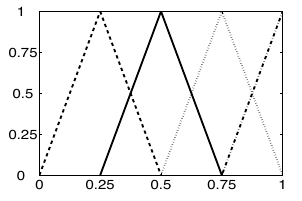
\includegraphics[width=\textwidth]{figures/ArbogastCoarse} \\
      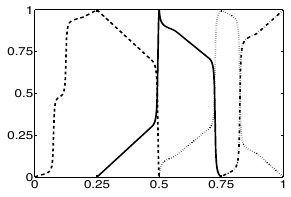
\includegraphics[width=\textwidth]{figures/ArbogastCoarseMs} \\
      {\small [Arbogast 2011]}
    \end{column}
    \begin{column}{0.6\textwidth}
      \begin{itemize}
      \item subassembly avoids explicit matrix triple product $A_{\text{coarse}} \gets P^T A_{\text{fine}} P$
      \item can update the coarse operator locally (e.g.~local nonlinearity)
      \item need not assemble entire fine grid operator
      \item if repetitive structure, need not store entire fine grid state
      \item can coarsen very rapidly (especially in smooth regions)
      \item lower communication setup phase
      \end{itemize}      
    \end{column}
  \end{columns}
\end{frame}

\begin{frame}{$\tau$ formulation of Full Approximation Scheme (FAS)}
  \begin{itemize}
  \item classical formulation: ``coarse grid \emph{accelerates} fine grid $\searrow \nearrow$
  \item $\tau$ formulation: ``fine grid feeds back into coarse grid'' $\nearrow \searrow$
  \item To solve $N u = f$, recursively apply
    \begin{equation*}
      \begin{split}
        \text{pre-smooth} \:\: & \quad \tilde u^h \gets S^h_{\text{pre}}(u^h_0, f^h) \\
        \text{solve coarse problem for $u^H$} \:\: & \quad N^H u^H = \underbrace{I_h^H f^h}_{f^H} + \underbrace{N^H \hat I_h^H \tilde u^h - I_h^H N^h \tilde u^h}_{\tau_h^H} \\
        \text{correction and post-smooth} \:\: & \quad u^h \gets S^h_{\text{post}} \Big( \tilde u^h + I_H^h (u^H - \hat I_h^H \tilde u^h), f^h \Big) \\
      \end{split}
    \end{equation*}
    \begin{tabular}{llll}
      \toprule
      $I_h^H$ & residual restriction & $\hat I_h^H$ & solution restriction \\
      $I_H^h$ & solution interpolation & $f^H = I_h^H f^h$ & restricted forcing \\
      $\{S^h_{\text{pre}},S^h_{\text{post}}\}$ & \multicolumn{3}{l}{smoothing operations on the fine grid} \\
      \bottomrule
    \end{tabular}
  \item At convergence, $u^{H*} = \hat I_h^H u^{h*}$ solves the $\tau$-corrected coarse grid equation
    $N^H u^H = f^H + \tau_h^H$,
    thus $\tau_h^H$ is the ``fine grid feedback'' that makes the coarse grid equation accurate.
  \item $\tau_h^H$ is \emph{local} and need only be recomputed where it becomes stale.
  \end{itemize}
\end{frame}

\begin{frame}{Cool Topics in Multiscale Computation}
  \begin{multicols}{2}
    \begin{itemize}
    \item Solve PDE in fewer flops than evaluating an analytic solution
    \item Solve PDE in $\bigO(\abs{\log n}\abs{\log \epsilon}^d)$ memory
    \item Compute $k$ eigenvalues in $\bigO(n \log k)$
    \item Project vector onto eigenbasis in $\bigO(n \log k)$
    \item Optimal-order graph partitioning and clustering
    \item Continuation and transient problems without revisiting fine grid
    \item Global optimization without sacrificing optimality, ``multiscale annealing''
    \item Accelerate Monte-Carlo slowdown due to spuriously correlated sampling
    \end{itemize}
  \end{multicols}
\end{frame}

\begin{frame}{Multilevel structure for uncertainty quantification}
  \centering
  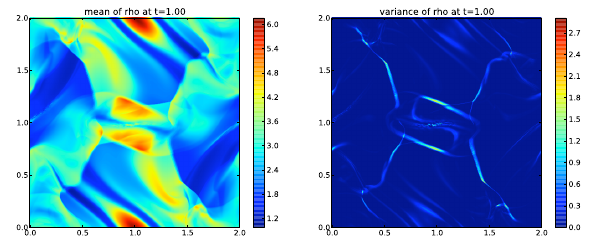
\includegraphics[width=0.9\textwidth]{figures/MG/MishraSchwabSukys2012OrszagTang}
  \begin{multicols}{2}
    \begin{itemize}\small
    \item Geometric hierarchy of models
    \item More samples on coarse grids (much cheaper)
    \item Mean and variance in $\sim 10\times$ cost of deterministic simulation
    \item Robust to dimension of stochastic space
    \end{itemize}
    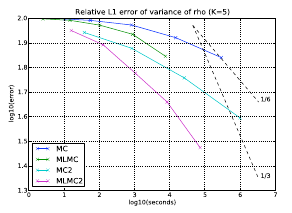
\includegraphics[width=0.45\textwidth]{figures/MG/MishraSchwabSukys2012OrszagTangTimeVariance}
  \end{multicols}
  {\scriptsize [Mishra, Schwab, {\v{S}}ukys, 2012]}
\end{frame}


\begin{frame}{Outlook}
  \begin{itemize}
  \item Multiscale processes are ubiquitous and important
  \item Multiscale computation necessary for modern simulation and analysis
  \item Embrace multiscale structure, make it work for you
  \item Raise level of abstraction at which we formulate problems
  \item Think in terms of robust functionals and statistics \\ rather than pointwise solutions
  \item Multiscale computation often reveals modeling flaws, \\
    guides their rectification
  \item Good microscale models are important for deriving and correcting coarse models
  \end{itemize}
\end{frame}

\end{document}
